This section documents the results of various experiments we did. Since the final aim of the
project is to predict breast cancer data accurately, we systematically tested all necessary components to perform this task, such that we ensure correctness (and reproducibility) of our final results. All plots show the performance of the model on testing data only.

\subsection{Linear Regression with Gradient Descent Methods}
We began with the most simple method, plain gradient descent, which we used with a constant learning rate. We tested the values $\eta \in \{ 0.1, 0.01, 0.001, 0.0001\}$ to find the best possible value to fixate for our experiments\footnote{The plots showing our testing can be found on GitHub in the directory \texttt{figures/all\_plots}.}, and based on this test, we saw that we had the best results when $\eta = 0.1$. With this as our learning rate, we studied convergence speed towards the minimum when using plain gradient descent and plain gradient descent with momentum. The plot showing this (as well as a comparison to the analytical solution) can be seen in figure \ref{fig:plainVSanalytical}, up to 10 epochs \cite{mediumEpochNumber}\cite{epochsBreastCancerArticle}.
\begin{figure}
    \centering
    \includegraphics[width=0.5\linewidth]{figures/all_plots/plain_mse_per_iter_eta_1e-1.png}
    \caption{Plain gradient descent (PGD) with and without momentum compared to the analytical solution, with a constant learning rate of $\eta = 0.1$ and a momentum parameter $\gamma = 0.5$.}
    \label{fig:plainVSanalytical}
\end{figure}

Next, we looked at our stochastic methods, with and without momentum. In this case we tried a linearly decaying learning rate to see if we would have any major improvements over plain gradient descent. In this case, the linearly decaying learning rate used was:
\[
\eta_t = (1- \frac{t}{5})0.01 + \frac{t}{5} 0.0001
\]
where we found the value $\eta_0 = 0.1$ after a few tests, as well as consulting the literature. We also kept the mini-batch size fixed at 4, which we found to produce decent values in this case. The comparison of the MSE with and without momentum as a function of epochs is displayed in figure \ref{fig:sgdVSanalytical}. 
\begin{figure}
    \centering
    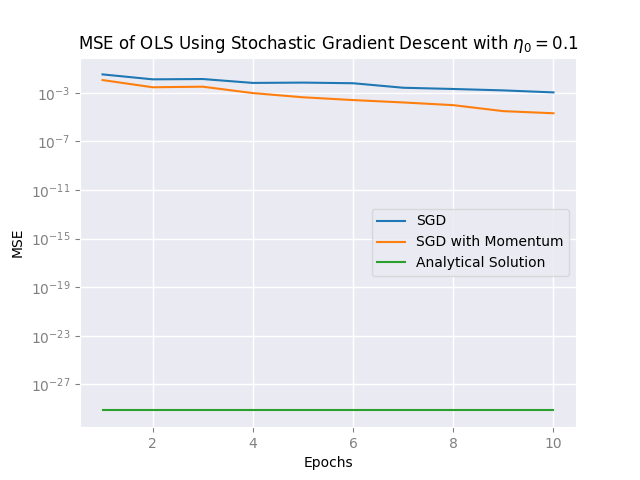
\includegraphics[width=0.5\linewidth]{figures/all_plot/sgd_mse_pr_epoch_eta_1e-1.png}
    \caption{Stochastic gradient descent (SGD) with and without momentum compared to the analytical solution, with a constant learning rate of $\eta_0 = 0.1$ and a momentum parameter $\gamma = 0.5$. The size of the mini-batches is also fixed at 4.}
    \label{fig:sgdVSanalytical}
\end{figure}

We timed our methods, and as expected, stochastic gradient descent gave us results quicker, with minimal detriment to the MSE. \textcolor{red}{(We should time our results with plain and SGD and mention here that SGD is quicker.)} From this point on, we will therefore continue using stochastic instead of plain gradient descent for computational efficiency.

Next, we looked at the methods with adaptive learning rates. All methods were initialized with the same global learning rate $\eta = 0.1$ to begin with, as this was the best result in both of our previous tests. We wanted to see how the different methods adapted the learning rate over time, and if this behavior was consistent with the theory. The learning rates as a function of epochs can be seen in figure \ref{fig:learningratesGD}, and the development of the MSE over epochs in figure \ref{fig:MSEGD}. We expect smoother graphs with faster convergence in methods with momentum, \textcolor{red}{true/false}.
\begin{figure}
    \centering
    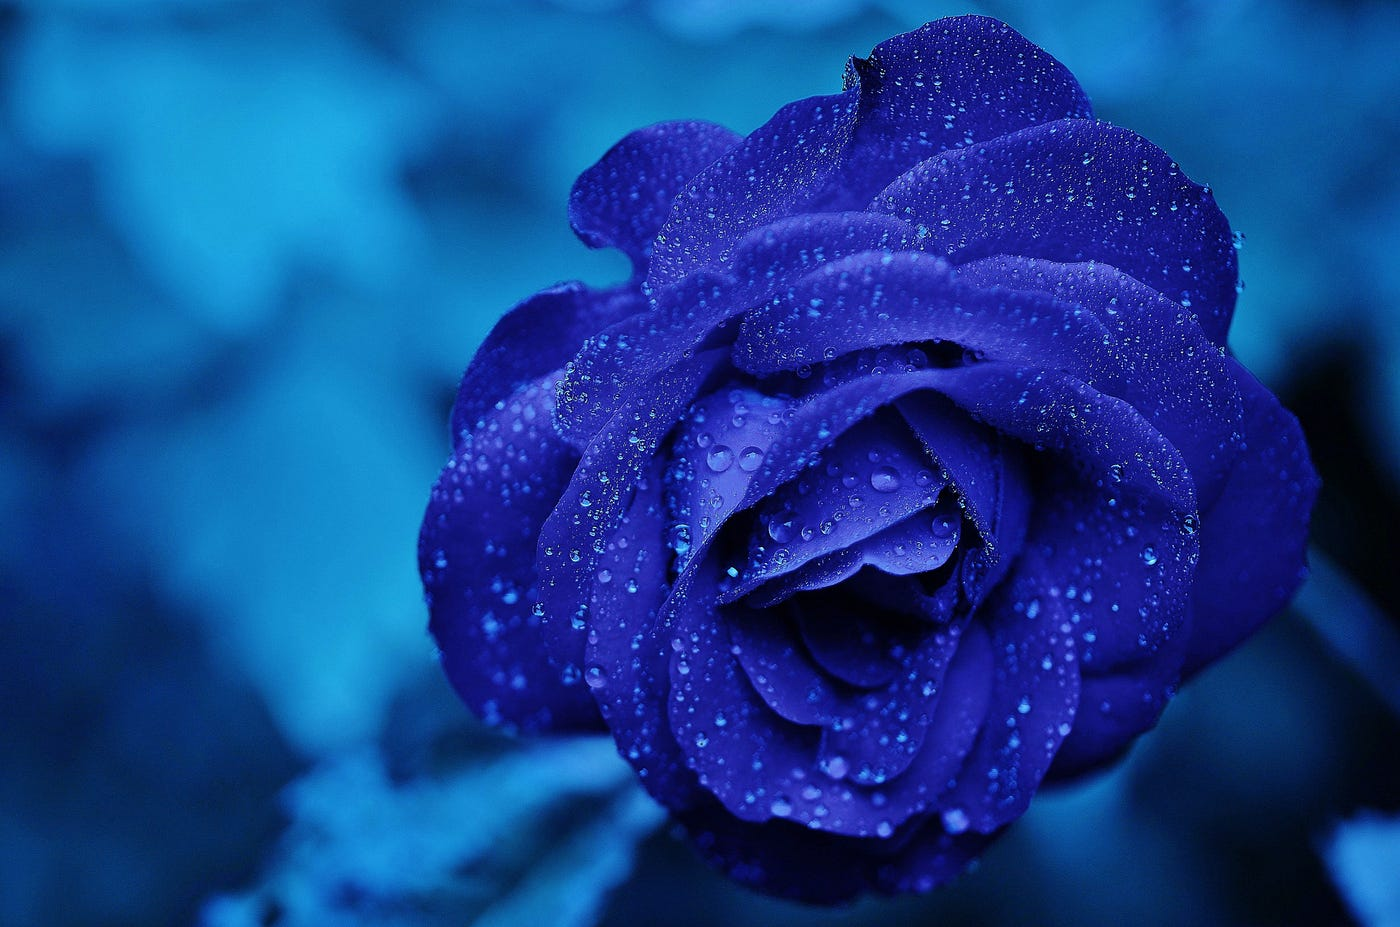
\includegraphics[width=0.5\linewidth]{figures/placeholders/learningratesGD.png}
    \caption{\textcolor{purple}{Plot of 3 subplots showing SGD w and w/o momentum for each of the three methods of adaptable learning rates.  Function of number of epochs. Learning rate on y-axis. See photo on Emma's phone.}}
    \label{fig:learningratesGD}
\end{figure}

\begin{figure}
    \centering
    
\includegraphics[width=0.5\linewidth]{figures/placeholders/MSEGD.png}
    \caption{\textcolor{purple}{Plot of 3 subplots showing SGD w and w/o momentum for each of the three methods of adaptable learning rates.  Function of number of epochs. MSE on y-axis.}}
    \label{fig:MSEGD}
\end{figure}

As part of our testing process, we compared the performance of our gradients to that of the automatic differentiation library Autograd \cite{autograd}. Since our tests pass\footnote{Tests can be found on our GitHub: \url{https://github.com/emmastorberg/FYS-STK4155_Project2/blob/main/tests.py}}, we expected our implementations to give quite similar results as these pre-existing methods, which they did\footnote{Plot showing our methods compared to Autograd can be found in appendix \textcolor{red}{(LETTER)}.}. 

Up to this point, we have only looked at OLS. When we use ridge regression instead, there is the additional hyperparameter $\lambda$ to consider. We performed a grid search to determine what combination of $\lambda$ and gradient descent method to choose, and tested $\lambda \in \text{\textcolor{red}{(value)}}$ against each of the seven methods we tested for OLS in figures \ref{fig:learningratesGD} and \ref{fig:MSEGD}. The grid search table can be seen in figure \ref{fig:gridsearch_ridge}, where we can visually determine the best method as \textcolor{red}{(add method here)}, with $\lambda = \text{\textcolor{red}{(value)}}$. \textcolor{red}{An additional table showing the results of a grid search for finding the best $R^2$ score can be found in appendix (LETTER). (Remove if we don't do this.)} 
\begin{figure}
    \centering
    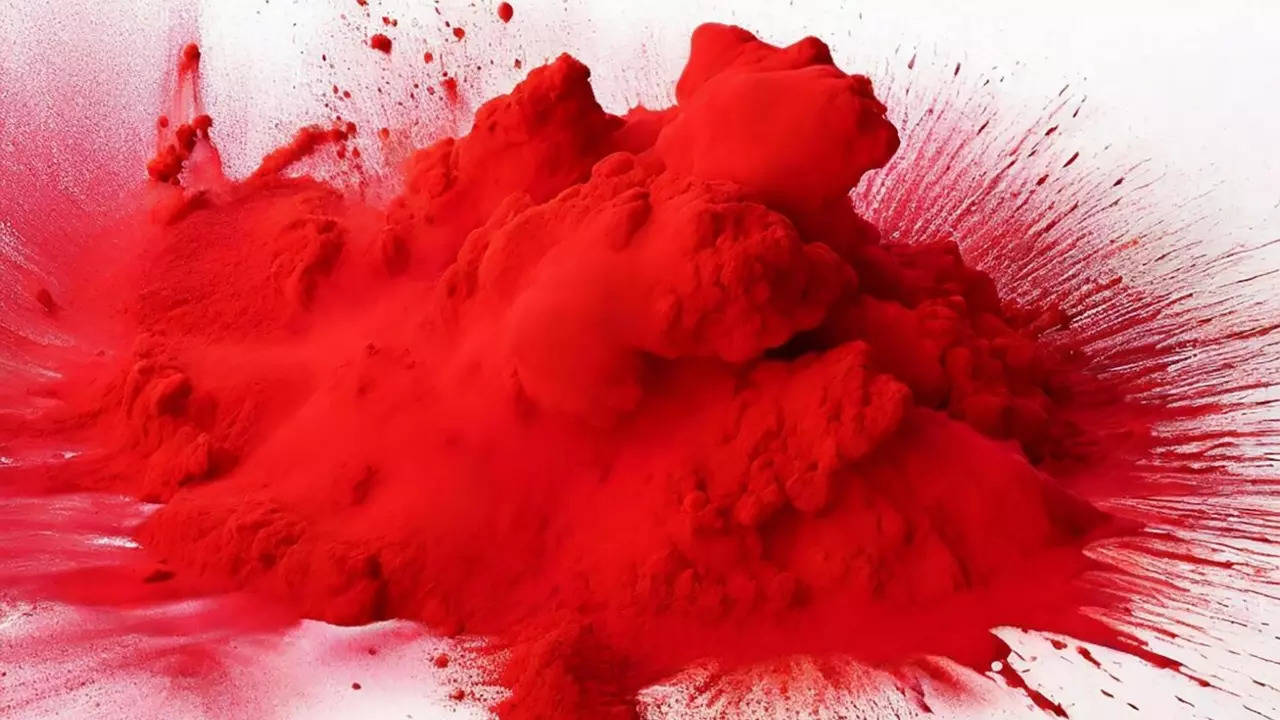
\includegraphics[width=0.5\linewidth]{figures/placeholders/gridsearch_ridge.png}
    \caption{\textcolor{purple}{Grid search table of the seven possible methods compared for different values of the hyperparameter $\lambda$}}
    \label{fig:gridsearch_ridge}
\end{figure}

\subsection{Numerical Prediction with Neural Network}
We saw that the optimal gradient descent methods for linear regression were \textcolor{red}{(method)} and \textcolor{red}{(method)}, with $\lambda = \text{\textcolor{red}{(value)}}$ for ridge regression. There is an enormous number of possible neural networks we can create even with only the relatively few gradient descent methods and activation functions at our disposal, in addition to the limitation of computation time. We eliminated a few degrees of freedom here by sticking to \textcolor{red}{(method)} as our gradient descent method (based on its performance in the experiments up to this point), and with ReLU as the activation function for the outer layer, guided by the theoretical intuition of what values it can produce (only positive values; the range of our polynomial $f(x) = \text{\textcolor{red}{(polynomial)}}$ is positive real numbers only).

To construct the network, we tried to sequentially eliminate degrees of freedom by fixating certain parameters, and thereafter exploring slight modifications to these. We started by using the same number of nodes per layer, and performing a grid search to find the best combination. The results of this are shown in figure \ref{fig:gridsearch_numpred_layers_nodes}, with sigmoid activating all hidden layers, and ReLU on the output layer.
\begin{figure}
    \centering
    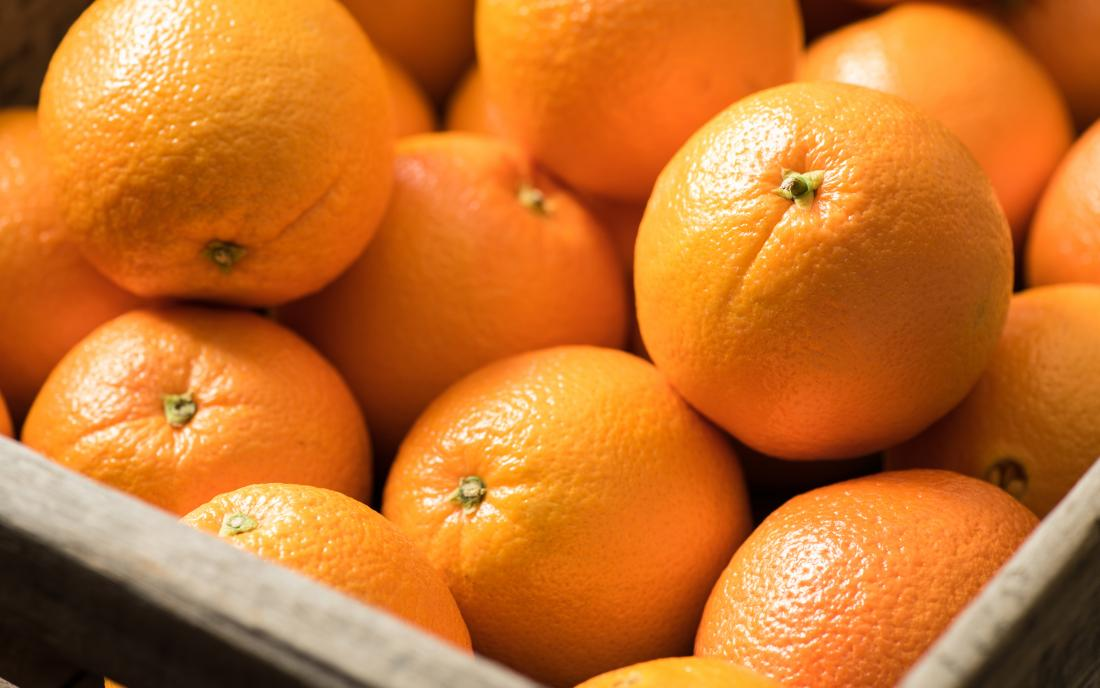
\includegraphics[width=0.5\linewidth]{figures/placeholders/gridsearch_numpred_layers_nodes.png}
    \caption{\textcolor{purple}{Heat map showing the MSE for the numerical NN predictions, as a function of hidden layers (1-5) and nodes in each hidden layer (1-10)}}
    \label{fig:gridsearch_numpred_layers_nodes}
\end{figure}

As we can see, a network with \textcolor{red}{(nodes and layers)} works the best out of the options we tested. Next, we tried varying what activation functions to use on the hidden layers. The plot of the resulting MSEs is shown in figure \ref{fig:activationfunctions_cost_numpred}. It seems clear that \textcolor{red}{(activation function)} activating the hidden layers is best in this case, so a neural network with \textcolor{red}{(NN explained here)} became the basis for further modifications in hopes of improving performance. 
\begin{figure}
    \centering
    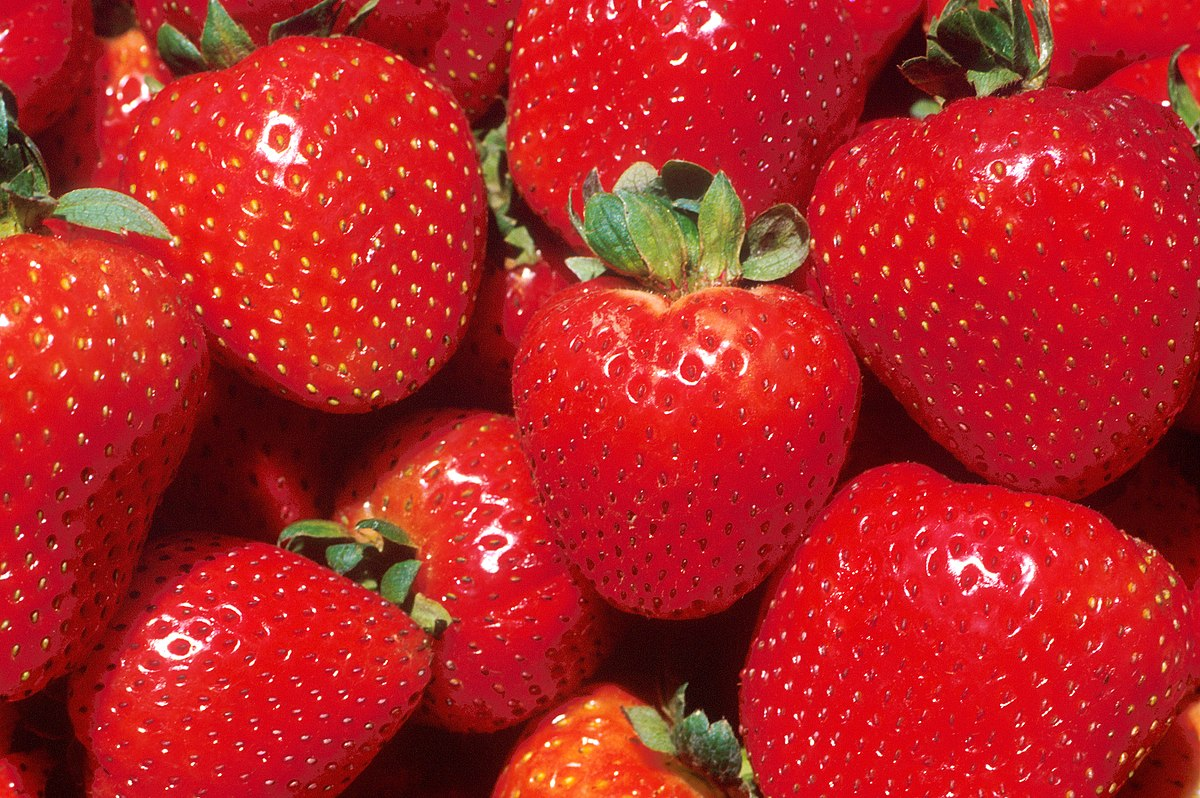
\includegraphics[width=0.5\linewidth]{figures/placeholders/activationfunctions_cost_numpred.png}
    \caption{\textcolor{purple}{Cost as a function of number of epochs, testing for four different neural networks. They all have the size determined in the grid search, but now we want to see if changing the activation of the hidden layers gives us any improvements.}}
    \label{fig:activationfunctions_cost_numpred}
\end{figure}

With slight variations to the hidden layers, the number of nodes in them and what activation functions to use at each stage, we arrived at our best-performing network for this task. The hyperparameters used to create it can be seen in table \ref{tab:numericalprediction}: 
\begin{table}[h!]
  \centering
  \small
  \begin{tabular}{|c|c|}
    \hline
    \textbf{Hyperparameter} & \textbf{Value} \\
    \hline
    Number of data points & $n = $ \\
    \hline
    Scaling of data & \texttt{StandardScaler} \\
    \hline
    Number of mini-batches (epochs) & $M =$ \\
    \hline
    Mini-batch size & $\frac{n}{M} = $ \\
    \hline
    Gradient descent method & Adam \\
    \hline
    Initial learning rate & $\eta = $ \\
    \hline
    Decay rate of first moment & $\rho_1 =$ \\
    \hline
    Decay rate of second moment & $\rho_2 = $ \\
    \hline
    Numerical stability constant & $\delta = $ \\
    \hline
    Cost function & MSE \\
    \hline
    Input layer & Size, activation \\
    \hline
    Layer 2 & Size, activation \\
    \hline
    Layer 3 & Size, activation \\
    \hline
    Output layer & Size, activation \\
    \hline
  \end{tabular}
  \caption{The chosen hyperparameters for best performance in numerical prediction task.}
  \label{tab:numericalprediction}
\end{table}

The neural network described \textcolor{blue}{above} was able to predict with an accuracy of \textcolor{red}{(value)}\%. The MSE of our best-performing neural network, OLS and ridge regression compared to a neural network created with Scikit-Learn can be seen in figure \ref{fig:numericalprediction}; a similar comparison of $R^2$ score can be found in figure \ref{fig:numericalpredictionR2} in appendix \textcolor{red}{(LETTER)}.

\begin{figure}
    \centering
    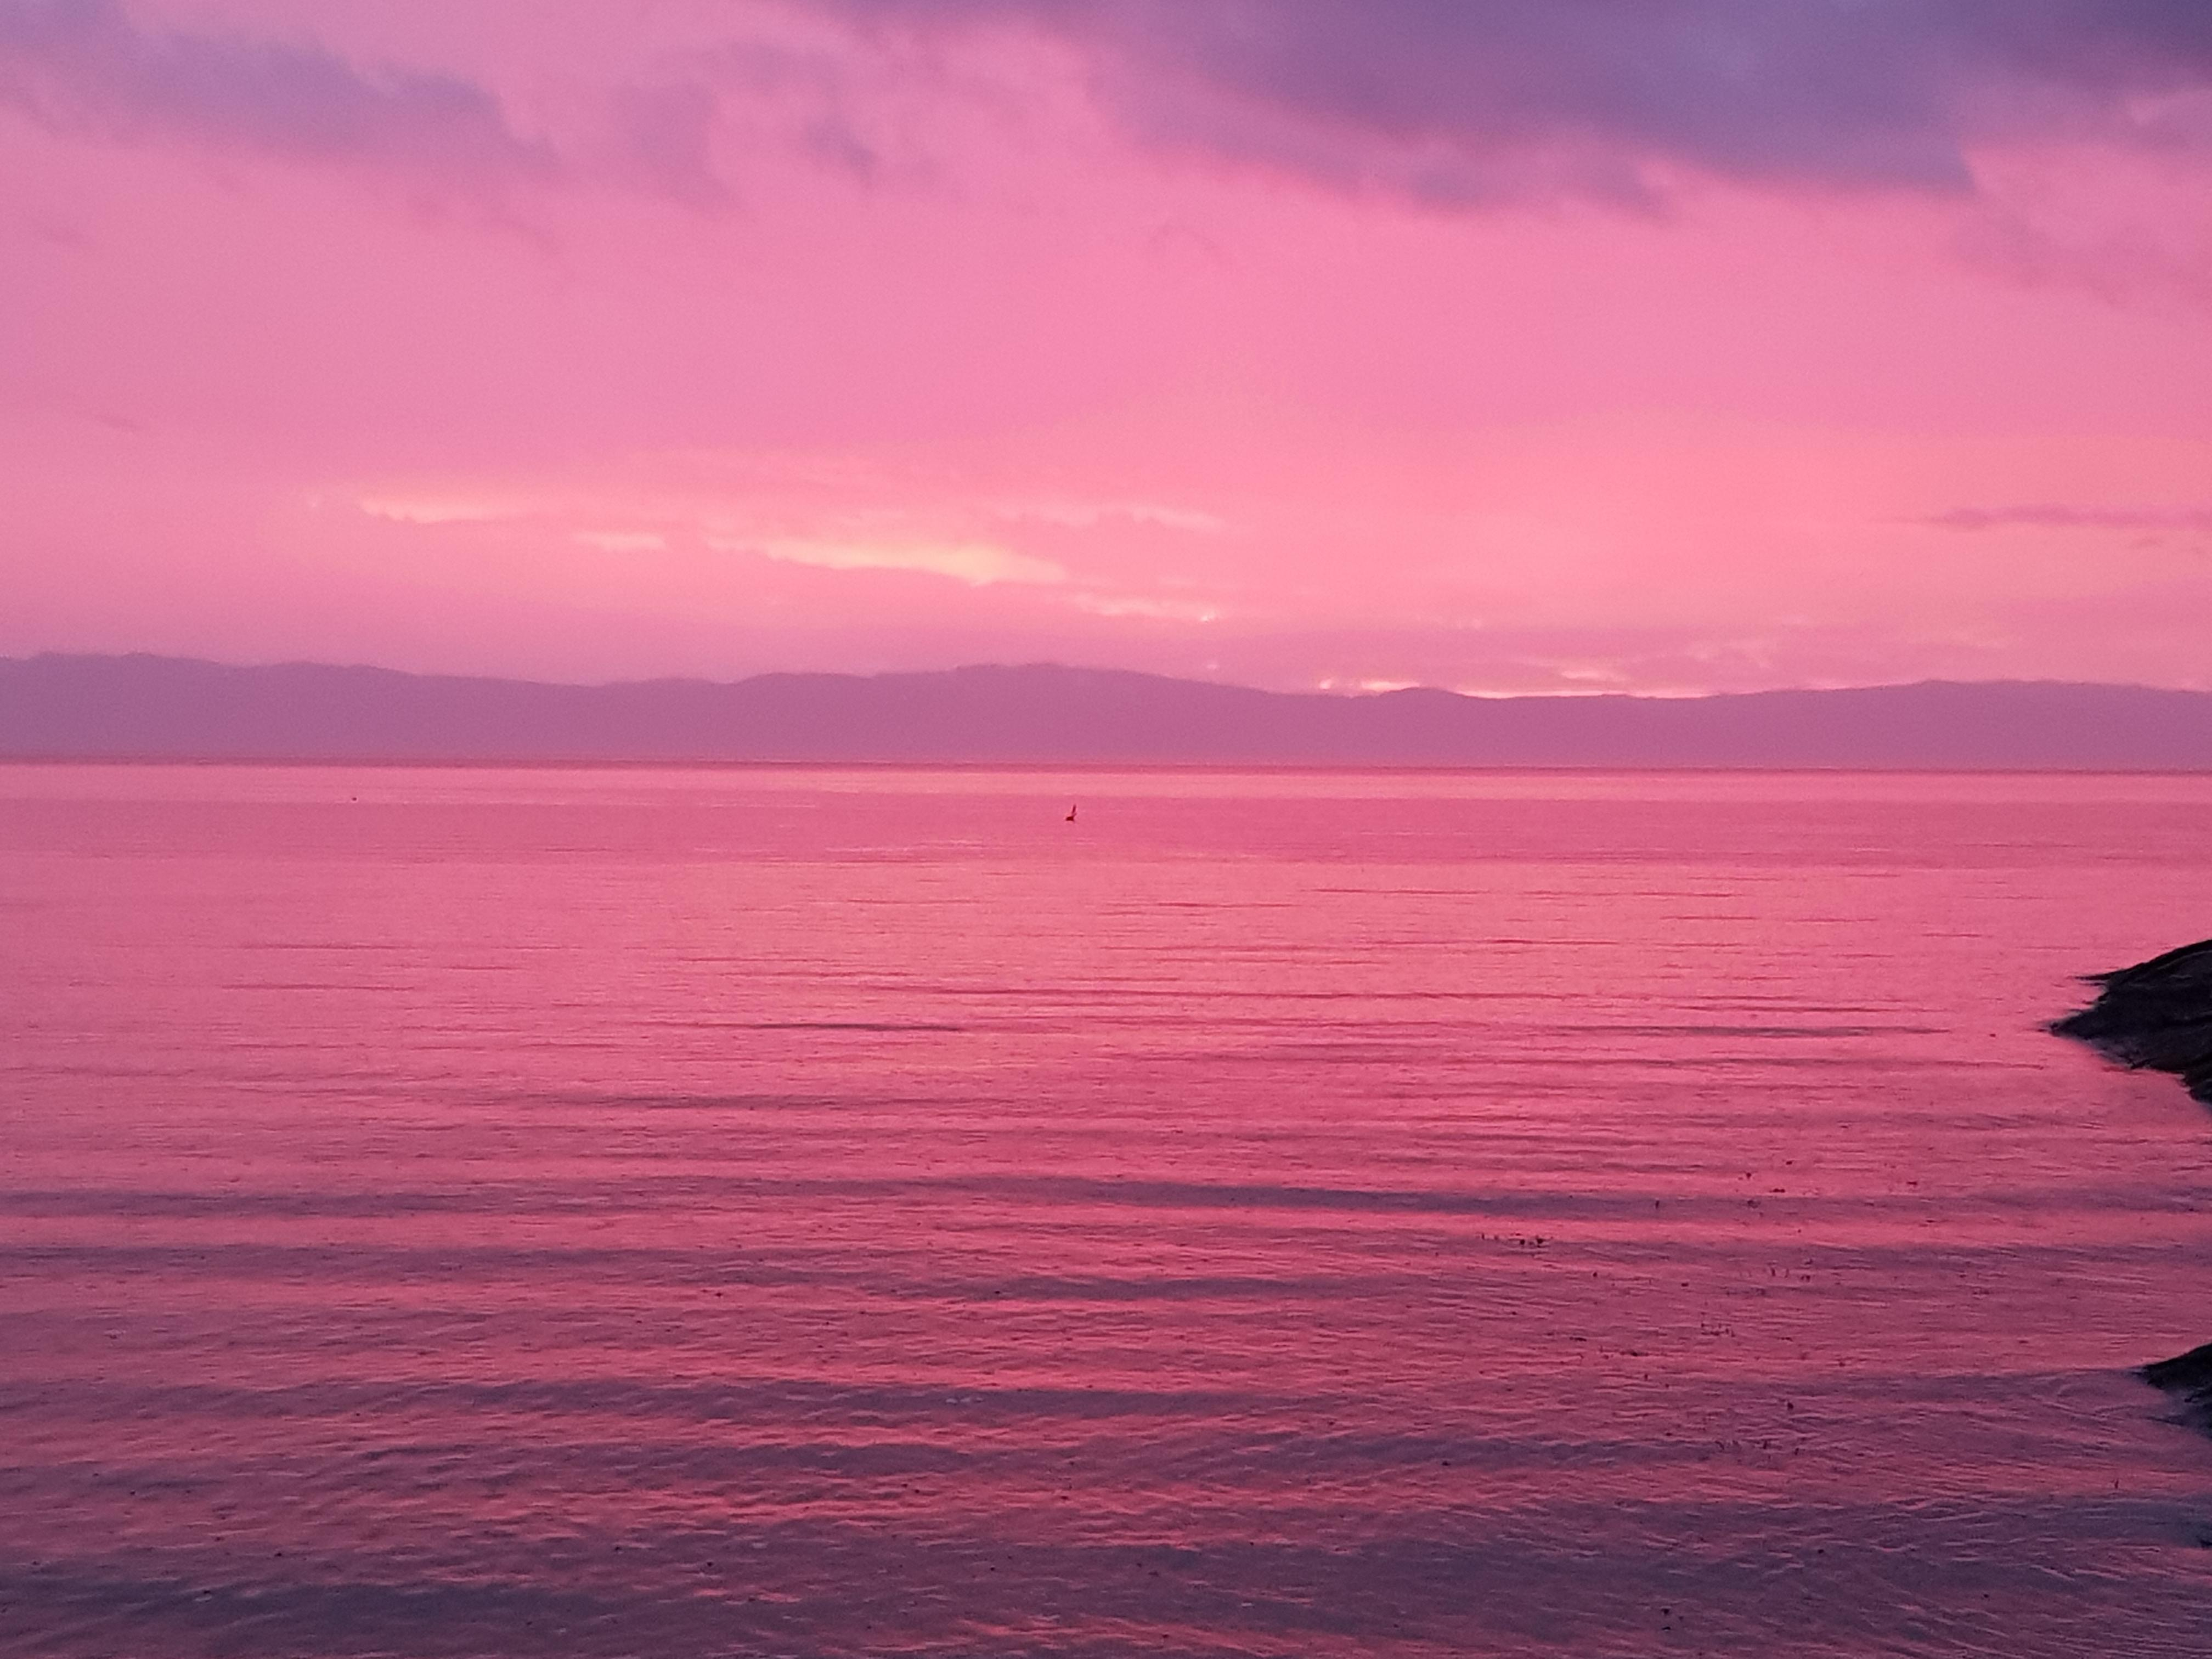
\includegraphics[width=0.5\linewidth]{figures/placeholders/numericalprediction.png}
    \caption{\textcolor{purple}{MSE as a function of epochs for OLS, Ridge and neural network (optimal version of all three methods). We also need a sklearn comparison here.}}
    \label{fig:numericalprediction}
\end{figure}

As we can see, it seems that the best method overall for this task is \textcolor{red}{(method)} with parameters \textcolor{red}{(parameters)}. 

\subsection{Classification with Neural Network}
Moving on to the classification task, we once again faced the issue of an extreme number of possibilities to test in order to construct the best-performing network. We limited our scope to only \textcolor{red}{(method)} with parameters \textcolor{red}{(parameters)}.

\subsubsection{First Attempt with Our Own Implementation}
Similar to the procedure in the creation of a network for numerical prediction, to make the optimal network for binary classification, we first employed a grid search of a fixed number of nodes per layer, and thereafter we altered the activation function on the hidden layers to see what gave the best results. In this process, we uncovered an error in the implementation. It looked as though the network predicted the average of the target vector, which gave an accuracy approximately equal to the frequency of target value 1 since we are working with binary classification. 

The source of the error, as well as its solution, remains elusive. We studied the implementation and behavior of our network extensively. Unit testing also passes for all of our methods\footnote{See our GitHub: \url{https://github.com/emmastorberg/FYS-STK4155_Project2}}.  

We initially scaled our data with \texttt{StandardScaler}, which we thought might be the issue, but changing the scaling to \texttt{MinMaxScaler} (also from Scikit-Learn \cite{sklearnScaling}) offered only an incremental change (from an accuracy of approximately 0.62 to 0.63). All gradient descent methods had also passed rigorous unit testing, and we also knew from the experiments in the previous section on the numerical prediction task that our neural network code was capable of producing reasonable results from a theoretical standpoint. 

We tested our network on different datasets, including the iris dataset \cite{irisdataset}, which is a common and beginner-friendly dataset used for testing classification networks. Our implementation performs well on this dataset when scaled with \texttt{StandardScaler}, though not with \texttt{MinMaxScaler}. This showed that it was able to do some classification tasks, so we hoped the implementation was not the problem, but rather that the choice of parameters happened to lead us to a local minimum, which is why the accuracy stopped improving at an early iteration. However, an identical instantiation with PyTorch, an optimized tensor library for deep learning \cite{pytorch}, creates a network that is able to classify the data points without issue, so the instantiation and choice of parameters is most likely not the problem.

These confusing findings left us with an unclear path towards analyzing our code implementation on breast cancer data, as was the goal of this project. We found that through trial and error, we could achieve accuracy as high as \textcolor{red}{(accuracy)} \%. However, seeing as this is a multiclass rather than binary classification problem, continuing to work with this network and dataset will leave us unable to compare our results to a logistic regression, nor will we be exploring the application of machine learning methods in the medical field, as was our initial motivation.

Therefore we ultimately made the decision to continue working with the breast cancer data using PyTorch to explore the optimal instantiation of a network for such a dataset. The resulting neural network will also be compared to a logistic regression. 

\subsubsection{Continued Exploration with PyTorch}
Our search for the optimal set of hyperparameters for the task was in part systematic, and in part educated guesswork and trial and error. The first systematic test was a grid search, where we fixed the number of nodes in each layer. Throughout this task, we always used sigmoid as the activation function. A grid search table showing the best combination of number of layers and nodes per layer (with sigmoid activating all layers) is shown in figure \ref{fig:gridsearch_layers_nodes}. 

% our final activation function, and kept the activation functions of the hidden layers the same. Of our four options, having \textcolor{red}{(activation function)} activate all hidden layers resulted in highest accuracy overall. 

\begin{figure}
    \centering
    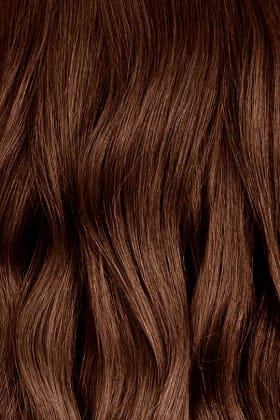
\includegraphics[width=0.5\linewidth]{figures/placeholders/gridsearch_layers_nodes.png}
    \caption{\textcolor{purple}{Heat map showing the accuracy for the neural net (on the cancer dataset), as a function of hidden layers (1-5) and nodes in each hidden layer (1-10)}}
    \label{fig:gridsearch_layers_nodes}
\end{figure}

As we can see, the optimal result seems to be \textcolor{red}{(nodes in each layer explained here)}. Using this as a starting point for further exploration, we continued looking into if a different set of activation functions for the hidden layers would have any effect. In figure \ref{fig:activationfunctions_cost}, we see all four options for activation functions on a neural network with \textcolor{red}{(nodes in each layer explained here)}, as determined in figure \ref{fig:gridsearch_layers_nodes}. We see that \textcolor{red}{(activation function)} works \textcolor{red}{better/worse} than our initial test using sigmoid everywhere, so we continued tweaking a network in the form of \textcolor{red}{best finding here}.

\begin{figure}
    \centering
    
\includegraphics[width=0.5\linewidth]{figures/placeholders/activationfunctions_cost.png}
    \caption{\textcolor{purple}{Cost as a function of number of epochs, testing for four different neural networks. They all have the size determined in the grid search, but now we want to see if changing the activation of the hidden layers gives us any improvements.}}
    \label{fig:activationfunctions_cost}
\end{figure}

Through less organized trial and error testing, we began with the optimal network so far, with size \textcolor{red}{(layer and node info)} and \textcolor{red}{(activation function)} on all hidden layers. We were able to find that with \textcolor{red}{(activation function on hidden layers)} and \textcolor{red}{(alternative neural network structure)}, we could now achieve an accuracy of up to \textcolor{red}{(accuracy)}\% for the Wisconsin Breast Cancer dataset. \textcolor{green}{We expected from the theory that ReLU would do well, and in particular, offer faster convergence than the other methods. This applies/does not apply in this case as well.} The full set of chosen hyperparameters for this neural network are shown in table \ref{tab:classificationtask}.

\begin{table}[h!]
  \centering
  \small
  \begin{tabular}{|c|c|}
    \hline
    \textbf{Hyperparameter} & \textbf{Value} \\
    \hline
    Number of data points & $n = $ \\
    \hline
    Scaling of data & \texttt{StandardScaler} \\
    \hline
    Number of mini-batches (epochs) & $M =$ \\
    \hline
    Mini-batch size & $\frac{n}{M} = $ \\
    \hline
    Gradient descent method & Adam \\
    \hline
    Initial learning rate & $\eta = $ \\
    \hline
    Decay rate of first moment & $\rho_1 =$ \\
    \hline
    Decay rate of second moment & $\rho_2 = $ \\
    \hline
    Numerical stability constant & $\delta = $ \\
    \hline
    Cost function & Cross-entropy \\
    \hline
    Input layer & Size, activation \\
    \hline
    Layer 2 & Size, activation \\
    \hline
    Layer 3 & Size, activation \\
    \hline
    Output layer & Size, activation \\
    \hline
  \end{tabular}
  \caption{Table showing hyperparameters chosen for best-performing neural network in classification task}
  \label{tab:classificationtask}
\end{table}
%\textcolor{magenta}{Figure: Activation functions. Plot the accuracy of the network (on cancer data) with different combinations of activation functions [leaky relu, relu, only sigmoid, softmax] (although I believe all should have sigmoid in the final layer), as a function of layers. (I think we should have a fixed number of nodes, unless we want to grid search this and choose the best)} \\ 
%\textcolor{purple}{Alternative figure to the one above. The same idea, but with the best layer and node size from the first heatmap/a grid search, as a function of epochs. This makes us able to visualize which activation function converges faster. I think this is a better plot} \\

%\textcolor{purple}{Figure: Accuracy for [SGD (with and without momentum), Adagrad (with and without momentum), RMSprop and Adam] (on the legend) as a function of epochs, with a fixed learning rate}
%We expect them to converge, some faster than others. With momentum should converge faster.

The network as described \textcolor{blue}{above} has \textcolor{red}{(accuracy)}\% accuracy in its predictions overall. However, we must also consider what type of inaccuracy is most prevalent before determining this is the best network for the task. False positive and negative rate can be seen in the confusion matrix in figure \ref{fig:confusionmatrix}.
\begin{figure}
    \centering
    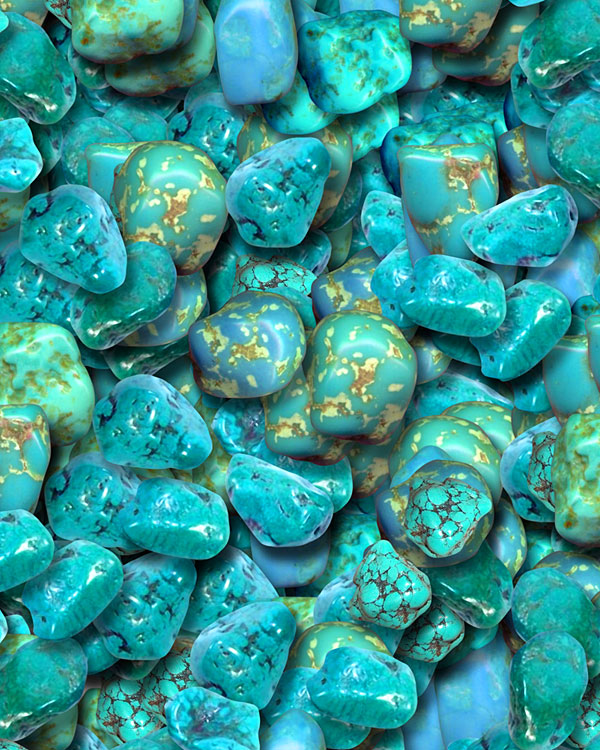
\includegraphics[width=\linewidth]{figures/placeholders/confusionmatrix.png}
    \caption{\textcolor{purple}{Confusion matrix for the neural net (on the cancer dataset, counting the number of TP, TN, FN and FP)}}
    \label{fig:confusionmatrix}
\end{figure}


\textcolor{red}{(Comment on FP and FN rate. If FP are higher than FN, our job is done and the results are good. If not, I (EMMA) think we need another plot showing tweaks we have made to prioritize having less FN. Check the text and code that I have commented out right below this.)}

% INCLUDE THIS PARAGRAPH IF ANOTHER PLOT IS NECESSARY; OTHERWISE, MOVE TO DISCUSSION.

% We tuned our model again to lower FN rate. The new confusion matrix can be shown in figure \ref{fig:confusionmatrix2}.
% \begin{figure}
%     \centering
%     
\includegraphics[width=0.5\linewidth]{figures/placeholders/confusionmatrix2.png}
%     \caption{\textcolor{purple}{Second confusion matrix for the neural net (on the cancer dataset, counting the number of TP, TN, FN and FP). Should definitely have less FN than FP this time around.}}
%     \label{fig:confusionmatrix2}
% \end{figure}

\subsection{Classification with Logistic Regression}
As discussed, an alternative to a neural network requiring far less tuning is logistic regression. This corresponds to a network with no hidden layers, activated by the sigmoid function. The resulting confusion matrix is shown in figure \ref{fig:logreg}. 
\begin{figure}
    \centering
    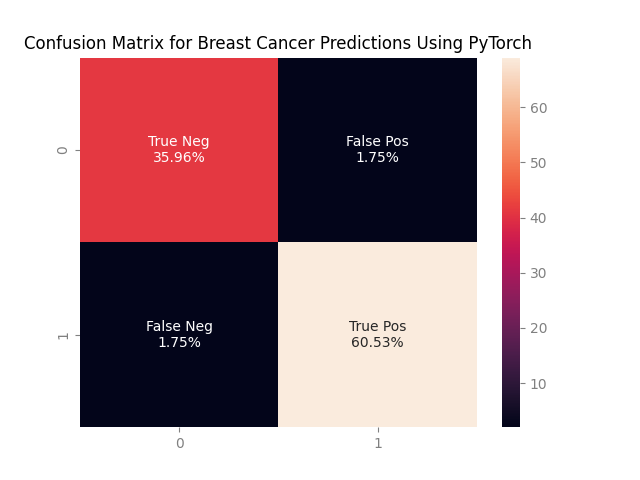
\includegraphics[width=0.5\linewidth]{figures/plots/logreg.png}
    \caption{\textcolor{purple}{Confusion matrix from logistic regression}}
    \label{fig:logreg}
\end{figure}

As we can see, the performance of logistic regression alone is relatively poor compared to a neural network. However, we experienced first-hand that it requires much less time to set up and run, which should be taken into account when evaluating these methods.

\textcolor{magenta}{Should not be in report, but we should print accuracy/cf before and after scaling with the StandardScaler. Expect accuracy to increase. We can just cite on of our previous reports on scaling with StandardScaler}



